\chapter{复数}
\section{引言——数系的发展与复数的起源}
数的概念及运算是从生产和科学研究的实践中产生和发展起来的。截至目前,同学们学过的数系是下表中实线画出的部分:
\begin{center}
    \begin{tikzpicture}[>=stealth]
\node (A) at (0,.5)[text width=1.5cm, align=center]{复数集\\($\mathbb{C}$)}; 
\node (B1) at (1.6,1.5)[text width=1.5cm, align=center]{实数集\\($\mathbb{R}$)}; 
\node (B2) at (1.6,-.5)[text width=1.5cm, align=center]{虚数集}; 
\node (C1) at (2.3,2.5)[right, text width=1.5cm, align=center]{有理数集\\($\Q$)}; 
\node (C2) at (2.3,1)[right, text width=5cm, align=center]{无理数集——无限不循环小数}; 
\node (D1) at (5,3)[text width=1.5cm, align=center]{整数集\\($\Z$)}; 
\node (D2) at (5,2)[text width=1.5cm, align=center]{分数集}; 
\node (E1) at (6.75,4)[text width=1.5cm, align=center]{自然数集\\($\N$)}; 
\node (E2) at (6.75,3.25)[text width=1.5cm, align=center]{零}; 
\node (E3) at (6.75,2.5)[text width=1.5cm, align=center]{负数}; 
\node (F1) at (9,3)[text width=2.5cm, align=center]{循环小数\\(包括整数和有限小数)}; 
\draw[decorate, decoration={brace, amplitude=8pt}, dashed](1,-.5)--(1,1.75);
\draw[decorate, decoration={brace, amplitude=5pt}](2.5,1)--(2.5,2.75);
\draw[decorate, decoration={brace, amplitude=5pt}](4.35,2)--(4.35,3.25);
\draw[decorate, decoration={brace, amplitude=5pt}](6,2.25)--(6,4.5);
\draw[decorate, decoration={brace, amplitude=5pt}](7.75,4.5)--(7.75,1.75);
    \end{tikzpicture}
    \end{center}

正如表中所列出的,从正整数(自然数)集$\N$到实数集$\R$,数系已经经历了三次扩充(下表中实箭头表示的部分)。本章将研究第四次扩充(虚箭头表示的部分):
\begin{center}
\begin{tikzpicture}[>=stealth]
\node(A) at (0,0)[text width=2cm, align=center]{正整数集\\($\N$)} ;
\node(B) at (6,0)[text width=1.5cm, align=center]{整数集\\($\Z$)} ;
\node(C) at (10,0)[text width=1.5cm, align=center]{有理数集\\($\Q$)} ;

\node(D) at (4,-1.5)[text width=1.5cm, align=center]{实数集\\($\R$)} ;
\node(E) at (8,-1.5)[text width=1.5cm, align=center]{复数集\\($\mathbb{C}$)} ;

\draw[->](A)--node[text width=4cm, align=center]{第I次\\引进零和负数}(B);
\draw[->](B)--node[text width=2cm, align=center]{第II次\\引进分数}(C);
\draw[->](D)--node[text width=2cm, align=center]{第IV次\\引进虚数}(E);
\draw[->](0,-1.5)--node[text width=2cm, align=center]{第III次\\引进无理数}(D);
\end{tikzpicture}
\end{center}


“温故知新”,让我们先回顾一下前三次扩充的事实和规律.

\subsection{从数集上的元素看}
数集的每次扩充都是在原有数集的基础上引入新数,构造出一个新数集,且使原有的数集成为新数集上的一个真子集。也就是说,数集以\textbf{逐次包含}的方式扩充。

\subsection{从数集上的运算看}
在新数集上我们这样定义新的运算法则:一方面要使新法则运用到原有数集上时必须与原有数集上的运算结果相一致;另一方面我们还希望新法则能使原数集上的运算规律保持不变。例如,在有理数集上计算$(+5)+(+6)$的结果应与在算术(正有理数集)中计算$5+6$的结果相一致,而且我们还希望在算术中对加法和乘法成立的交换律、结合律和分配律能在有理数集上保持不变。也就是说,在原来数集上成立的算律,在扩充后的数集上希望它能继续成立。这是很重要的\textbf{数集扩充的原则}。

\subsection{从数集扩充的动力看}
数集的每次扩充既是度量的需要(这一点大家比较清楚),又是数学理论发展的需要(特别是解方程的需要)。例如:

方程$x+4=0$在自然数集上无解,而在扩充后的整数集上有唯一解$x=-4$;

方程$5x=3$,在整数集上无解,而在扩充后的有理数集
上有唯一解$x=\frac{3}{5}$(若不扩充数集,连这种最简单的一元一
次方程的理论也不能完整)。

方程$x^2=2$在有理数集上无解,在扩充后的实数集上有两个解$x=\pm\sqrt{2}$.

最早呼唤扩充实数集的问题是解二次方程。事实上,在实数集上不能提供二次方程的完整理论。如方程
\begin{equation}
    x^2=-1 \tag{1}
\end{equation}
在实数集上就没有解,因为任意实数的平方都不可能为负数。

摆在人们面前有两种选择:要么宣布方程(1)无解;要么沿着数集扩充的方向朝前走——引入新数,扩充实数集,使方程(1)有解。一些严峻的事实迫使人们选择了后者。于是在16世纪中叶,人们开始引入一个由等式
\begin{equation}
    i^2=-1  \tag{2}
\end{equation}
所定义的新数$i$(它显然不是实数)\footnote{$i$是英文单词imaginaries(虚的)的字头,瑞士大数学家欧拉首先用它表示虚数单位.
},它被称做虚数单位。这样,方程(*)至少有了一个根$i$。进而,根据数集扩充的原则,我们还规定实数可以和它进行四则运算,并且进行四则运算时,原有的加、乘算律仍然成立。于是自然造出了诸如$2i$, $3i$, $2+5i$这样一些新数。

应该指出:引进的新数$i$以及上面造出的形如$a+bi$($a,b\in\R$)的数,起初人们对它感到迷惑不解,特别是当$b\ne 0$时,认为这些都是“虚假的数”[这是因为当时人们习惯于把数作为某种计数手段,然而形如$a+bi\; (a,b\in\R,\; \text{且}b\ne 0)$的新数却起不到计数手段的作用],“虚数”正是由此而得名。

虚数诞生后,除了用来表示方程的解以外,一时尚找不
到更多的应用,因此发展十分缓慢。到了18世纪末叶,维塞尔(Wessel)、阿尔纲(Argand)和高斯(Gauss)几乎同时给这些新数以几何解释(见6.2节)以后,才在数学、物理的应用和研究中逐渐有了越来越多且越来越重要的用途,这进一步推动了人们研究的兴趣。19世纪初,高斯把形如$a+bi\; (a,b\in\R)$的数称为复数。如果说微积分的研究统治了18世纪的话,那么,19世纪数学家们的兴奋中心便是关于复数理论及其应用的研究。现在复数已经发展成为一门十分重要的基础数学分支——复变函数论,它是数学、物理和技术科学中有力的数学工具之一。

本章将学习复数的初步知识。

\section{复数的概念}
\subsection{复数的定义}
在引言中我们已经看到,虚数单位$i$是由等式
$i^2=-1$
定义的。形如$a+bi\; (a,b\in\R)$的数称为\textbf{复数},一般用小写字母$z$表示,即$z=a+bi\; (a,b\in\R)$,$a$与$b$分别叫做$z$的\textbf{实部}[记作$R(z)$]与\textbf{虚部}[记作$I(z)$]. 全体复数构成的集合称为\textbf{复数集},一般用大写字母$\mathbb{C}$来表示\footnote{$C$是英语词组Complex numbers(复数)的第一个字母。}.

对于复数$z=a+bi\; (a,b\in\R)$:
\begin{itemize}
    \item 当$b=0$时,$z$就是实数;
    \item 当$b\ne 0$时,$z$叫做\textbf{虚数};
    \item 当$a=0$,且$b\ne 0$时,$z$叫做\textbf{纯虚数}。
\end{itemize}
以上事实还可以用“充要条件”的记号表示为:

\noindent
\begin{minipage}{.55\textwidth}
\[\begin{split}
    a+bi\in\R &\Longleftrightarrow b=0\\
    a+bi\text{是虚数}&\Longleftrightarrow b\ne 0\\
    a+bi\text{是纯虚数}&\Longleftrightarrow a=0\text{且}b\ne 0\\
\end{split}  \]
由此可以看出:实数集和虚数集都是复数集的真子集(图6.1)
\end{minipage}\hfill
\begin{minipage}{.4\textwidth}
\centering
\begin{tikzpicture}[scale=1.2]
\draw[pattern=north east lines](0.5,0.5) rectangle (4.5,3);
\draw[thick](1.5,1.5)node[fill=white]{\small 纯虚数集} circle (.8);
\draw[thick, fill=white](3.5,1.5)node{\small 实数集} circle (.8);
\node at (2.5,2.6)[fill=white]{\small 虚集};
\end{tikzpicture}
\captionof{figure}{}
\end{minipage}

\begin{example}
    已知$z=(m^2-3m-4)+(m-5)i$,其中$m\in\R$,试求$m$为何值时,
\begin{multicols}{3}
\begin{enumerate}[(1)]
\item $z\in\R$;    \item $z$是虚数;    \item $z$是纯虚数。 
\end{enumerate}
\end{multicols}
\end{example}


\begin{analyze}
由$m\in\R \Rightarrow (m^2-3m-4)\in\R,\; (m-5)\in\R$, 以下应根据复数分类的充要条件来解。
\end{analyze}

\begin{solution}
\begin{enumerate}[(1)]
    \item $\because\quad b=0\Rightarrow z\in\R$
    
$\therefore\quad  m-5=0$,可得$m=5$.
    \item $\because\quad b\ne 0\Rightarrow z$是虚数,
    
$\therefore\quad m-5\ne 0$,得$m\ne 5$.
    \item $\because\quad \begin{cases}
        a=0\\ b\ne 0
    \end{cases} \Rightarrow z$是纯虚数,

$\therefore\quad  \begin{cases}
    m^2-3m-4=0\\m-5\ne 0
\end{cases}\Longleftrightarrow \begin{cases}
    m=4\text{或}m=-1\\
    m\ne 5
\end{cases}$

$\therefore\quad m=4$或$m=-1$.
\end{enumerate}

\end{solution}

\subsection{复数相等的定义}
若两个复数$z_1=a+bi\; (a,b\in\R)$与$z_2=c+di\; (c,d\in\R)$的实部与虚部分别相等,称这两个\textbf{复数相等},记作$z_1=z_2$,即
\[a+bi=c+di  \Longleftrightarrow a=c\text{且}b=d\]
由此可见,一个复数对应唯一的有序实数对$(a,b)$,反之亦然。

\begin{thm}
{推论1} \[a+bi=0\Longleftrightarrow a=0\text{且}b=0\]
\end{thm}

\begin{thm}
{推论2}\[a+bi\ne c+di\Longleftrightarrow a\ne c\text{或}b\ne d\]
\end{thm}

\begin{example}
    已知$(2x-1)+(3-x)i=x-(3+y)i$,其中$x,y\in\R$,求$x$与$y$。
\end{example}

\begin{analyze}
    由$x,y\in\R\Rightarrow (2x-1)\in\R,\;  (3-x)\in\R,\; (3+y)\in\R$,以下可用复数相等的定义转化成方程组来解。
\end{analyze}

\begin{solution}
    由已知条件
\[\begin{cases}
    2x-1=x\\ 3-x=-(3+y)
\end{cases} \Rightarrow \begin{cases}
    x=1\\ y=-5
\end{cases}\]
\end{solution}

应该理解:当给出两个复数相等这样的条件时,就意味着在实数集上能获得两个独立条件。

\subsection{复数在平面上的表示}
引言告诉我们,复数的几何解释的出现是使复数能在数学和物理中得以应用的极为重要的原因,也是复数发展史上的转折点,本节开始研究复数的几何解释。

由复数相等的定义可以看出,任何一个复数$z=a+bi\; (a,b\in\R)$对应唯一的有序实数对$(a,b)$,而有序实数对$(a,b)$又对应直角坐标系(笛卡儿坐标系)上的唯一的点$Z(a,b)$(图6.2),由此想到,点$Z(a,b)$的位置可以形象地用来表示复数$z=a+bi$,而且这种表示是唯一的(图6.3)。这种用来表示复数的平面称为\textbf{复平面}(也叫\textbf{高斯平面}),在
高斯平面上,$x$轴叫做\textbf{实轴},$y$轴除去原点后的部分叫做\textbf{虚轴}(因为原点表示实数0,所以原点不能在虚轴上)。

\noindent
\begin{minipage}{.45\textwidth}
    \centering
\begin{tikzpicture}[>=stealth, scale=.8]
\draw[->](-1,0)--(3,0)node[below]{$x$};
\draw[->](0,-1)--(0,3)node[left]{$y$};
\node[below left]{$O$};
\draw(2,0)node[below]{$a$}--(2,2.5)node[above right]{$Z(a,b)$}--(0,2.5)node[left]{$b$};

\end{tikzpicture}  
\captionof{figure}{}
\end{minipage}\hfill
\begin{minipage}{.45\textwidth}
\centering
\begin{tikzpicture}[>=stealth, scale=.8]
    \draw[->](-1,0)--(3,0)node[below]{$x$};
    \draw[->](0,-1)--(0,3)node[left]{$y$};
    \node[below left]{$O$};
    \draw(2,0)node[below]{$a$}--(2,2.5)node[above right]{$z=a+bi$}--(0,2.5)node[left]{$b$};
\end{tikzpicture}    
\captionof{figure}{}
\end{minipage}

\begin{ex}
\begin{enumerate}
    \item 在复平面上回答:
\begin{enumerate}[(1)]
\item 表示实数的点集构成的图形是\blank\blank ;
\item 表示虚数的点集构成的图形是\blank\blank ;
\item 表示纯虚数的点集构成的图形是\blank\blank .
\end{enumerate}

    \item 数集$\mathbb{C}$与复平面上的点集之间的对应是\blank\blank .
    \item 在复平面上图示满足$1\le R(Z)\le 3$,且$1< I(Z)\le 2$的点$Z$构成的图形.
\end{enumerate}   
\end{ex}

\subsection{共轭复数}
实部相等,虚部为相反数的两个复数称作\textbf{共轭复数}(当虚部不为0时,也称\textbf{共轭虚数})。复数$z$的共轭复数记为$\bar z$。根据这个定义可以看出:

\noindent
\begin{minipage}{.55\textwidth}
\begin{enumerate}[(1)]
\item 若$z=a+bi,\; (a,b\in\R)$,则$\bar z=a-bi$,

$\bar{\bar z}=\overline{a-bi}=a+bi$,即$\bar{\bar z}=z$
\item 在复平面上,表示两个互为共轭的复数$z$与$\bar z$的点关于实轴对称(图6.4)。
\item 不难证明:$z\in\R \Longleftrightarrow \bar z=z$
\end{enumerate}
\end{minipage}\hfill
\begin{minipage}{.4\textwidth}
\centering
\begin{tikzpicture}[>=stealth, scale=.8]
    \draw[->](-1,0)--(3,0)node[below]{$x$};
    \draw[->](0,-2)--(0,2)node[left]{$y$};
    \node[below right]{$O$};
    \draw[dashed](0,1.5)--(2,1.5)node[right]{$z=a+bi$}--(2,-1.5)node[right]{$\bar z=a-bi$}--(0,-1.5);
\foreach \x in {-1.5,1.5}
{
    \draw[fill](2,\x)circle (1.5pt);
}
\end{tikzpicture}   
\captionof{figure}{} 
\end{minipage}

\subsection{虚数无大小顺序}
我们知道,两个实数可以比大小。但是两个虚数之间是不能比大小的,虚数与实数之间也不
能比大小。关于这两个命题的证明本书从略。

\section*{习题一}
\begin{center}
    \bfseries A
\end{center}

\begin{enumerate}
    \item 说出下列复数中,哪些是实数,哪些是纯虚数,哪些是虚数:
    \[ 0.618,\; \frac{2}{7}i,\; 0,\; i,\; i^2,\; 2+3i,\; 2+\sqrt{7},\; 
    5i+8,\; 3-9\sqrt{2}i,\; i^2(1-\sqrt{3}),\; 3-\sqrt{5}i\]
    \item 说出下列复数的实部与虚部:
    \[-5+\sqrt{3}i,\; \frac{\sqrt{2}}{2}-\sqrt{3}i,\; -i,\; 0,\; -\sqrt{3},\; 8i-4\]
    \item 说出图中复平面上的点$Z_1,Z_2,\ldots,Z_8,Z_9$所表示的复数。
\begin{figure}[htp]
    \centering
\begin{tikzpicture}[>=stealth, scale=.5]
\draw[->](-6,0)--(6.5,0)node[below]{$x$};
\draw[->](0,-5)--(0,4)node[left]{$y$};
\draw[step=1, gray, thin](-5,-4) grid(5,3);    
\node [below left]{$O$};
\tkzDefPoints{2/3/Z_1, 3/1/Z_2, 2/0/Z_3, 0/-2/Z_4, -4/0/Z_5, 0/2/Z_6, -2/1/Z_7, -3/-3/Z_8, 2/-4/Z_9}
\tkzDrawPoints(Z_1,Z_2,Z_3,Z_4,Z_5,Z_6,Z_7,Z_8,Z_9)
\tkzLabelPoints[right](Z_1, Z_2, Z_6, Z_7, Z_4)
\tkzLabelPoints[above](Z_3,Z_9)
\tkzLabelPoints[below](Z_5, Z_8)
\foreach \x in {1,2,3}
{
    \node at (\x,0)[below]{$\x$};
    \node at (0,\x)[left]{$\x$};
}
\end{tikzpicture}
    \caption*{第3题}
\end{figure}

\item 在复平面内描出表示下列复数的点。
\[z_{1}=2+5i,\; z_{2}=-3+2i,\; z_{3}=\frac{1}{2}-3i,\; z_{4}=-i-3,\; z_{5}=5,\]
\[z_{6}=-4i,\; z_{7}=3i,\; z_{8}=-\sqrt{3}\]
\item 设$z=a+bi\; (a,b\in \R)$, 当$a,b$满足什么条件时,表示复
数$z$的点才能位于(口答):
\begin{multicols}{2}
\begin{enumerate}[(1)]
\item 实轴上;
\item 虚轴上;
\item 上半平面(不包括实轴);
\item 右半平面(不包括虚轴和原点).
\end{enumerate}
\end{multicols}

\item 说出下列复数的共轭复数,并在复平面内把每对共轭复
数表示出来。
$$z_{1}=4-3i,\; z_{2}=-1+i,\; z_{3}=-5-2i,\; z_{4}=4i-2,\; z_{5}=5,\; z_{6}=-3i$$
\item 说出复数 $2,\pi,0,-\frac13$的共轭复数。
\item 判断下列命题的真假,并说明理由。
\begin{enumerate}[(1)]
\item 设$z=a+bi\; (a,b\in \R)$, 当$a=0$时,$z$是纯虚数;
\item 原点是复平面内实轴与虚轴的公共点;
\item 实数的共轭复数一定是实数,虚数的共轭复数一定
是虚数。
\end{enumerate}
\item 填空:
\begin{enumerate}[(1)]
\item 若把复数集$\mathbb{C}$看做全集,那么$\R$的补集是\blank\blank ; 
\item 实数集与虚数集的交集是\blank\blank ;
\item 纯虚数集是虚数集的\blank\blank .
\end{enumerate}

\item $m\; (m\in\R)$取什么值时,复数$z=(m^2-3m-4)+(m^2-5m-6)i$是
\begin{multicols}{3}
\begin{enumerate}[(1)]
\item 实数;    \item 纯虚数;    \item 零。
\end{enumerate}

\end{multicols}

\item $m$是什么实数时,$z=(2+i)m^2-3(1+i)m-2(1-i)$是:
\begin{multicols}{4}
    \begin{enumerate}[(1)]
    \item 实数;  \item 虚数;  \item 纯虚数;    \item 零。
    \end{enumerate}
    
    \end{multicols}

\item 求适合下列条件的$x$与$y\; (x,y\in\R)$值:
\begin{multicols}{2}
 \begin{enumerate}[(1)]
\item $(3x-4)+(2y-1)i=0$;
\item $(x+y)-xyi=24i-5$;
\item $x^2-y^2+2xyi=8+6i$;
\item $(2x^2-5x+2)+i(y^2+y-2)=0$.
\end{enumerate}   
\end{multicols}
\end{enumerate}

\begin{center}
    \bfseries B
\end{center}

\begin{enumerate}\setcounter{enumi}{12}
    \item 已知$z_{1}=\sin2\theta+i\cos\theta$, $z_{2}=\cos\theta+i\sqrt{3}\sin\theta$, $\theta$取何值时:
\begin{multicols}{2}
\begin{enumerate}[(1)]
    \item $z_{1}=z_{2}$
    \item $z_{1}=\bar z_{2}$
\end{enumerate}
\end{multicols}
\item 证明: 
\begin{enumerate}[(1)]
\item    $z\in \R\Longleftrightarrow\overline{z}=z$; 
\item $z\text{为纯虚数}\Longleftrightarrow\overline{z}=-z\; (z\neq0)$。
\end{enumerate}
\item 在复平面上图示满足下列条件的复数$z$ 所 构成的图形。
\begin{multicols}{2}
\begin{enumerate}[(1)]
\item $0\leqslant I(z)<3$
\item $R(z)+I(z)=0$
\item $R(z)+2I(z)=1$
\item $[R(z)]^{2}+[I(z)]^{2}=2$  
\end{enumerate}
\end{multicols}

\item 用复数表示图中的用影区域:(见图)
\begin{figure}[htp]
    \centering
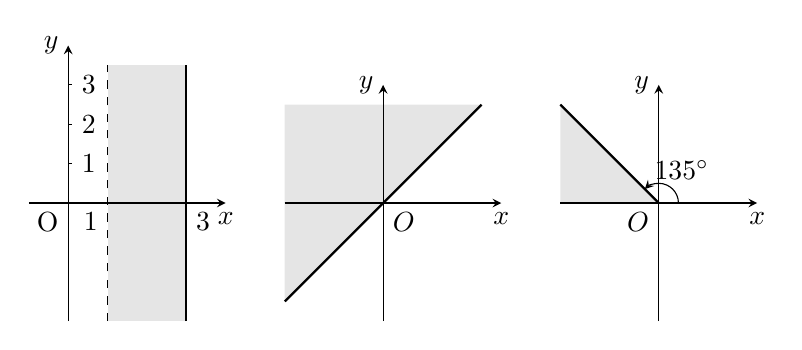
\begin{tikzpicture}[>=stealth, scale=.5]
\begin{scope}
    \fill[gray!20!white](1,-3) rectangle (3,3.5);
\draw[->](-1,0)--(4,0)node[below]{$x$};
\draw[->](0,-3)--(0,4)node[left]{$y$};
\foreach \x in {1,2,3}
{
    \draw(0,\x)--(.1,\x)node[right]{$\x$};
}

\draw[dashed](1,-3)--(1,3.5);
\draw[thick](3,-3)--(3,3.5);
\node[below left]{O};
\node at (1,0)[below left]{1};
\node at (3,0)[below right]{3};

\end{scope}
\begin{scope}[xshift=8cm]
    \fill[gray!20!white](-2.5,-2.5)--(-2.5,2.5)--(2.5,2.5)--cycle;
    \draw[->](-2.5,0)--(3,0)node[below]{$x$};
\draw[->](0,-3)--(0,3)node[left]{$y$};
\node[below right]{$O$};

\draw[thick](-2.5,-2.5)--(2.5,2.5);
\end{scope}
\begin{scope}[xshift=15cm]
    \fill[gray!20!white](-2.5,0)--(-2.5,2.5)--(0,0)--cycle;
    \draw[->](-2.5,0)--(2.5,0)node[below]{$x$};
\draw[->](0,-3)--(0,3)node[left]{$y$};
\node[below left]{$O$};
\draw[->](.5,0) arc (0:135:.5)node[above right]{$135^{\circ}$};
\draw[thick](-2.5,2.5)--(0,0);
\end{scope}
\end{tikzpicture}
    \caption*{第16题}
\end{figure}
\end{enumerate}



\subsection{复数的向量表示}
在物理学中,我们经常遇到力、速度、加速度、电场强度等,这些量,除了要考虑它们的绝对值的大小以外,还要考虑它们的方向,我们把这种既有绝对值大小又有方向的量叫做\textbf{向量}。向量可以用有向线段表示,线段的长度就是这个向量的绝对值(叫做这个\textbf{向量的模}),线段的方向(用箭头表示)就是这个向量的方向。模相等且方向相同的向量,不管它们的起点在哪里,都认为是\textbf{相等的向量}。在这一规定下,向量可以根据需要进行平移。模为零的向量(它的方向是任意的)叫做\textbf{零向量},规定所有的零向量相等。

\noindent
\begin{minipage}{.6\textwidth}\CTEXindent
复数可以用向量表示。前面我们已经看到
\[\text{复数集$\mathbb{C}$}\xleftrightarrow[]{\text{一一对应}}\text{复平面上的点集}\]
如图6.5中,复平面内点$Z(a,b)$表示复数$a+bi$,连接$OZ$,如果我们把有向线段$OZ$(方向是从原点$O$指向点$Z$)看成向量,记作$\VEC{OZ}$,这样就把复数同向量联系起来了。
\end{minipage}\hfill
\begin{minipage}{.35\textwidth}
\centering
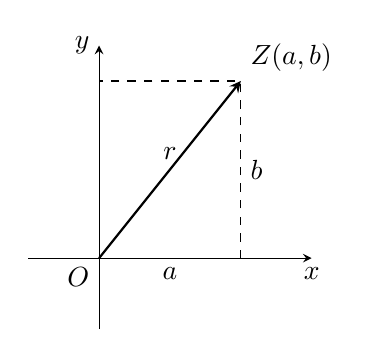
\begin{tikzpicture}[>=stealth, scale=.9]
    \draw[->](-1,0)--(3,0)node[below]{$x$};
    \draw[->](0,-1)--(0,3)node[left]{$y$};
    \node[below left]{$O$};
    \draw[dashed](2,0)--node[right]{$b$}(2,2.5)node[above right]{$Z(a,b)$}--(0,2.5);
\draw[->, thick](0,0)--node[above]{$r$}(2,2.5);
\node at (1,0)[below]{$a$};

\end{tikzpicture}   
\captionof{figure}{} 
\end{minipage}

很明显,从原点出发的向量$\VEC{OZ}$是由点$Z$所表示的复数唯一确定的;反过来,点$Z$所表示的复数也可以由从原点出发的向量$\VEC{OZ}$唯
一确定. 因此,复数集$\mathbb{C}$与复平面内所有以原点为起点的向量所成的集合也是一一对应的。此外,我们还规定,相等的向量表示同一个复数。

当$z=a+bi$用向量$\VEC{OZ}$表示时,
由于$\VEC{OZ}$的模(记作$|\VEC{OZ}|$)$r=\sqrt{a^2+b^2}$,于是,
我们也把$r$叫做\textbf{复数$a+bi$的模}(或\textbf{绝对值}),记作$|z|$或
$|a+bi|$. 因此有
\[|\VEC{OZ}|=|z|=|a+bi|=r=\sqrt{a^2+b^2}\]
其几何意义是复平面上表示复数$z$的点到原点的距离。

很有趣的是:当$b=0$时,$z=a+bi=a$, $|z|=|a|$,即$|z|$就是实数$a$的绝对值。可见,“复数的模(也叫复数的绝对值)”是实数的绝对值这一概念的扩充。
















